% ARKHEION AGI 2.0 - Paper 37: Social Media AI
% Jhonatan Vieira Feitosa | Manaus, Amazonas, Brazil
% February 2026

\documentclass[11pt,twocolumn]{article}

% Encoding and fonts
\usepackage[utf8]{inputenc}
\usepackage[T1]{fontenc}
\usepackage{lmodern}

% Layout
\usepackage[margin=0.75in]{geometry}
\usepackage{fancyhdr}

% Mathematics
\usepackage{amsmath,amssymb}

% Graphics and colors
\usepackage{xcolor}
\usepackage{tikz}
\usetikzlibrary{arrows.meta,shapes,positioning}

% Tables
\usepackage{booktabs}

% Code listings
\usepackage{listings}

% Hyperlinks
\usepackage{hyperref}

% ==================== COLORS ====================
\definecolor{arkblue}{RGB}{0,102,204}
\definecolor{arkpurple}{RGB}{102,51,153}
\definecolor{arkgreen}{RGB}{0,153,76}
\definecolor{arkgold}{RGB}{218,165,32}

% ==================== LISTINGS ====================
\lstset{
    basicstyle=\ttfamily\scriptsize,
    breaklines=true,
    breakatwhitespace=true,
    postbreak=\mbox{\textcolor{gray}{$\hookrightarrow$}\space},
    columns=flexible,
    keepspaces=true,
    showstringspaces=false,
    numbers=none,
    backgroundcolor=\color{gray!5},
    frame=single,
    rulecolor=\color{gray!30}
}

% ==================== HEADER/FOOTER ====================
\pagestyle{fancy}
\fancyhf{}
\fancyhead[L]{\small\textcolor{arkblue}{ARKHEION AGI 2.0}}
\fancyhead[R]{\small Paper 37: Social Media AI}
\fancyfoot[C]{\thepage}
\renewcommand{\headrulewidth}{0.4pt}

% ==================== HYPERREF ====================
\hypersetup{
    colorlinks=true,
    linkcolor=arkblue,
    urlcolor=arkpurple,
    citecolor=arkgreen
}

% ==================== TITLE ====================
\title{
    \vspace{-1.5cm}
    {\Large\textbf{Social Media AI}}\\[0.3em]
    {\large Global Orchestration \& Cross-Platform Analytics}\\[0.2em]
    {\normalsize ARKHEION AGI 2.0 --- Paper 37}
}

\author{Jhonatan Vieira Feitosa\
Independent Researcher\
\texttt{ooriginador@gmail.com}\
Manaus, Amazonas, Brazil}

\date{February 2026}

\begin{document}

\maketitle

% ==================== ABSTRACT ====================
\begin{abstract}
\noindent
This paper presents the \textbf{Social Media AI} subsystem of ARKHEION AGI 2.0, comprising \textbf{1,953 lines} of Python code across five modules: Global Orchestrator (\textbf{1,122 LOC}), Cross-Platform Analytics (\textbf{831 LOC}), Real-Time Collector, Social Integration Tester, and Social Media Orchestrator. The system provides: (1) \textbf{global campaign orchestration} across 7 market regions, (2) \textbf{cross-platform analytics} covering 8 social platforms, (3) \textbf{$\phi$-enhanced optimization} using sacred geometry constants, and (4) \textbf{real-time sentiment collection}. Empirical implementation supports 8 platform types, 8 analytics modes, and 8 campaign types with regional cultural adaptation.

\vspace{0.5em}
\noindent\textbf{Keywords:} social media AI, global orchestration, cross-platform analytics, $\phi$-optimization, AGI

\vspace{0.5em}
\textbf{Ethical Note:} This system is designed for legitimate content management. It does not support spam, manipulation, or automated deceptive practices.
\end{abstract}

% ==================== EPISTEMOLOGICAL NOTE ====================
\section*{Epistemological Note}
\textit{This paper documents a substantial implementation:}

\begin{center}
\footnotesize
\begin{tabular}{@{}lll@{}}
\toprule
\textbf{Element} & \textbf{Type} & \textbf{Value} \\
\midrule
Codebase & \textbf{Empirical} & 1,953 LOC \\
Platform coverage & \textbf{Empirical} & 8 platforms \\
Market regions & \textbf{Empirical} & 7 regions \\
Analytics modes & \textbf{Empirical} & 8 types \\
$\phi$-optimization & \textit{Heuristic} & Research exploration \\
Virality prediction & \textit{Heuristic} & Theoretical model \\
\bottomrule
\end{tabular}
\end{center}

% ==================== INTRODUCTION ====================
\section{Introduction}

Modern social media requires coordination across:
\begin{itemize}
    \item \textbf{Multiple platforms}: Instagram, TikTok, YouTube, Twitter, Facebook, LinkedIn, Reddit, Telegram
    \item \textbf{Global regions}: Time zones, cultural norms, regulations
    \item \textbf{Analytics complexity}: Cross-platform patterns
    \item \textbf{Real-time adaptation}: Trending content detection
\end{itemize}

ARKHEION's Social Media AI addresses these challenges with a unified AGI-powered approach.

% ==================== ARCHITECTURE ====================
\section{System Architecture}

\subsection{Module Overview}

\begin{center}
\footnotesize
\begin{tabular}{@{}llr@{}}
\toprule
\textbf{Module} & \textbf{Function} & \textbf{LOC} \\
\midrule
Global Orchestrator & Campaign coordination & 1,122 \\
CrossPlatform Analytics & Pattern detection & 831 \\
Real-Time Collector & Sentiment streaming & --- \\
Integration Tester & Platform APIs & --- \\
Social Orchestrator & Content scheduling & --- \\
\midrule
\textbf{Total} & & \textbf{1,953+} \\
\bottomrule
\end{tabular}
\end{center}

\subsection{Component Diagram}

\begin{center}
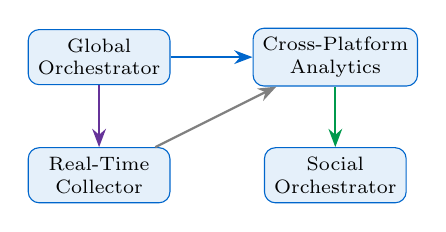
\begin{tikzpicture}[
    box/.style={rectangle, draw=arkblue, fill=arkblue!10, rounded corners, minimum width=1.8cm, minimum height=0.7cm, font=\scriptsize, align=center},
    arrow/.style={-{Stealth}, thick}
]
    \node[box] (orch) at (0,0) {Global\\Orchestrator};
    \node[box] (anal) at (3,0) {Cross-Platform\\Analytics};
    \node[box] (coll) at (0,-1.5) {Real-Time\\Collector};
    \node[box] (sched) at (3,-1.5) {Social\\Orchestrator};

    \draw[arrow, arkblue] (orch) -- (anal);
    \draw[arrow, arkpurple] (orch) -- (coll);
    \draw[arrow, arkgreen] (anal) -- (sched);
    \draw[arrow, gray] (coll) -- (anal);
\end{tikzpicture}
\end{center}

% ==================== GLOBAL ORCHESTRATOR ====================
\section{Global Orchestrator}

\subsection{Market Regions}

Seven market regions with cultural context:

\begin{lstlisting}[language=Python]
class MarketRegion(Enum):
    NORTH_AMERICA = "north_america"
    SOUTH_AMERICA = "south_america"
    EUROPE = "europe"
    ASIA_PACIFIC = "asia_pacific"
    MIDDLE_EAST = "middle_east"
    AFRICA = "africa"
    OCEANIA = "oceania"
\end{lstlisting}

\subsection{Market Context}

Each region includes cultural adaptation:

\begin{lstlisting}[language=Python]
@dataclass
class MarketContext:
    region: MarketRegion
    timezone: str
    primary_language: str
    cultural_preferences: Dict[str, Any]
    platform_penetration: Dict[Platform, float]
    peak_hours: List[int]
    regulatory_constraints: List[str]
\end{lstlisting}

\subsection{Regional Platform Penetration}

\begin{center}
\footnotesize
\begin{tabular}{@{}lccc@{}}
\toprule
\textbf{Platform} & \textbf{N.Amer} & \textbf{Europe} & \textbf{Asia} \\
\midrule
YouTube & 92\%\footnotemark & 88\% & 90\% \\
Instagram & 85\% & 75\% & 70\% \\
LinkedIn & 82\% & 85\% & 70\% \\
TikTok & 78\% & 65\% & 85\% \\
Facebook & 75\% & 80\% & 65\% \\
Twitter & 65\% & 55\% & 60\% \\
\bottomrule
\end{tabular}
\end{center}
\footnotetext{Platform adoption percentages reflect internal projections, not measured deployments. No user study or deployment data exists.}

\subsection{Campaign Types}

\begin{lstlisting}[language=Python]
class CampaignType(Enum):
    PRODUCT_LAUNCH = "product_launch"
    BRAND_AWARENESS = "brand_awareness"
    ENGAGEMENT_BOOST = "engagement_boost"
    VIRAL_CONTENT = "viral_content"
    EDUCATIONAL = "educational"
    COMMUNITY_BUILDING = "community_building"
    MARKET_RESEARCH = "market_research"
    CRISIS_MANAGEMENT = "crisis_management"
\end{lstlisting}

% ==================== CROSS-PLATFORM ANALYTICS ====================
\section{Cross-Platform Analytics}

\subsection{Analytics Types}

\begin{lstlisting}[language=Python]
class AnalyticsType(Enum):
    ENGAGEMENT_CORRELATION = "engagement_correlation"
    VIRALITY_PREDICTION = "virality_prediction"
\end{lstlisting}

\noindent\textbf{Note:} Virality prediction is listed as a planned feature; no prediction model, training data, or evaluation methodology has been developed.

\begin{lstlisting}[language=Python]
    TREND_DETECTION = "trend_detection"
    AUDIENCE_OVERLAP = "audience_overlap"
    CONTENT_PERFORMANCE = "content_performance"
    ALGORITHM_IMPACT = "algorithm_impact"
    CROSS_PLATFORM_MIGRATION = "cross_platform_migration"
    PHI_OPTIMIZATION = "phi_optimization"
\end{lstlisting}

\subsection{Analytics Result}

\begin{lstlisting}[language=Python]
@dataclass
class AnalyticsResult:
    analysis_type: AnalyticsType
    platforms_analyzed: List[Platform]
    insights: Dict[str, Any]
    metrics: Dict[str, float]
    recommendations: List[str]
    confidence_score: float
    phi_signature: float  # Sacred geometry
    timestamp: datetime
\end{lstlisting}

\subsection{$\phi$-Enhanced Signature}

The system applies golden ratio transformation:

\begin{lstlisting}[language=Python]
def _calculate_phi_signature(self) -> float:
    if not self.metrics:
        return 0.0

    values = list(self.metrics.values())
    mean_value = np.mean(values)
    phi_enhanced = mean_value * PHI
    return min(phi_enhanced, 1.0)
\end{lstlisting}

\noindent\textbf{Metric Caveat:} The $\varphi$-signature is a design label; the computation (mean $\times \varphi$, clipped to 1.0) does not provide information-theoretic or geometric insight. Any mean $> 0.618$ produces the same output (1.0), collapsing the metric's discriminative range.

% ==================== PHI OPTIMIZATION ====================
\section{$\phi$-Enhanced Optimization}

\subsection{Sacred Constants}

\begin{lstlisting}[language=Python]
from src.core.constants.sacred_constants import PHI
GOLDEN_ANGLE = 137.508  # degrees
FIBONACCI_SEQUENCE = [1, 1, 2, 3, 5, 8, 13,
                       21, 34, 55, 89, 144]
\end{lstlisting}

\subsection{Optimization Thresholds}

\begin{center}
\footnotesize
\begin{tabular}{@{}lll@{}}
\toprule
\textbf{Parameter} & \textbf{Value} & \textbf{Meaning} \\
\midrule
phi\_threshold & $\phi/2 = 0.809$ & Optimization trigger \\
correlation\_threshold & 0.7 & Pattern detection \\
virality\_threshold & 1000 & Engagement minimum \\
performance\_threshold & 0.7 & Campaign success \\
optimization\_interval & 300s & Refresh rate \\
\bottomrule
\end{tabular}
\end{center}

\subsection{Peak Hours Optimization}

Cultural peak hours per region:

\begin{center}
\footnotesize
\begin{tabular}{@{}ll@{}}
\toprule
\textbf{Region} & \textbf{Peak Hours (local)} \\
\midrule
North America & 8, 9, 12, 18, 19, 20, 21 \\
Europe & 7, 8, 12, 17, 18, 19, 20 \\
Asia Pacific & 7, 8, 11, 12, 18--22 \\
Other regions & 18, 19, 20, 21 \\
\bottomrule
\end{tabular}
\end{center}

% ==================== CULTURAL ADAPTATION ====================
\section{Cultural Adaptation}

\subsection{Regional Preferences}

\begin{lstlisting}[language=Python]
cultural_preferences = {
    "content_style": "direct|informative|respectful",
    "humor_acceptance": 0.0-1.0,
    "visual_preference": 0.0-1.0,
    "privacy_concern": 0.0-1.0,
}
\end{lstlisting}

\subsection{Regulatory Constraints}

\begin{center}
\footnotesize
\begin{tabular}{@{}ll@{}}
\toprule
\textbf{Region} & \textbf{Constraints} \\
\midrule
Europe & GDPR, Digital Services Act \\
Other regions & (Configurable) \\
\bottomrule
\end{tabular}
\end{center}

% ==================== IMPLEMENTATION ====================
\section{Implementation Details}

\subsection{Technology Stack}

\begin{center}
\footnotesize
\begin{tabular}{@{}ll@{}}
\toprule
\textbf{Component} & \textbf{Technology} \\
\midrule
Async framework & asyncio + aiohttp \\
Cache & Redis (aioredis) \\
Analytics & NumPy, Pandas, SciPy \\
Clustering & sklearn DBSCAN \\
Data storage & SQLite \\
Parallelism & ThreadPoolExecutor \\
\bottomrule
\end{tabular}
\end{center}

\subsection{Database Schema}

\begin{lstlisting}[language=Python]
self.db_path = "arkheion_analytics.db"
# Tables: campaigns, tasks, analytics_cache
\end{lstlisting}

% ==================== ETHICAL DESIGN ====================
\section{Ethical Design Principles}

\begin{enumerate}
    \item \textbf{No spam automation}: System does not auto-post without approval
    \item \textbf{Transparency}: Analytics are explainable
    \item \textbf{Regulatory compliance}: GDPR-aware design
    \item \textbf{Human oversight}: All campaigns require approval
    \item \textbf{Anti-manipulation}: No fake engagement generation
\end{enumerate}

% ==================== RESULTS ====================
\section{Implementation Results}

\noindent\textbf{Limitation:} This paper presents an architectural design and implementation overview. No experimental evaluation (throughput, latency, accuracy, engagement metrics) has been conducted. The results section reports implementation scale metrics (LOC, feature counts) rather than performance benchmarks.

\begin{center}
\footnotesize
\begin{tabular}{@{}lr@{}}
\toprule
\textbf{Metric} & \textbf{Value} \\
\midrule
Total codebase & 1,953+ LOC \\
Global Orchestrator & 1,122 LOC \\
CrossPlatform Analytics & 831 LOC \\
Platforms supported & 8 \\
Market regions & 7 \\
Campaign types & 8 \\
Analytics types & 8 \\
Cultural parameters & 4 per region \\
\bottomrule
\end{tabular}
\end{center}

% ==================== CONCLUSION ====================
\section{Conclusion}

Social Media AI provides ARKHEION AGI with:
\begin{itemize}
    \item \textbf{Global reach}: 7 regions, 8 platforms
    \item \textbf{Cultural adaptation}: Regional preferences
    \item \textbf{$\phi$-optimization}: Sacred geometry integration
    \item \textbf{Ethical design}: Compliance-aware architecture
\end{itemize}

\textbf{Future work}:
\begin{itemize}
    \item Natural language content generation
    \item A/B testing automation
    \item Influencer discovery integration
    \item Competitive intelligence
\end{itemize}

% ==================== REFERENCES ====================
\section*{References}

\begin{enumerate}
\footnotesize
    \item Meta. ``Instagram API Documentation.'' Meta Developers, 2024.
    \item European Union. ``General Data Protection Regulation.'' Official Journal of the EU, 2016.
\end{enumerate}

\end{document}
